\chapter{Charakteristická impedancia a odrazy na dlhom vedení}

\lettrine{K}{oaxiálny} kábel prenášajúci signál v kmitočtovom pásme stoviek $\un{MHz}$ predstavuje dlhé vedenie ($l \geq \frac{\lambda}{4}$), \cite{tirpak} teda také, ktoré nemožno modelovať sústredením jeho parazitných parametrov do diskrétnych prvkov. Napätie i prúd sú preto funkciami času aj polohy; merné (na jednotku dĺžky) primárne parametre v prípade homogénneho vedenia nie sú funkciami polohy. Pozdĺžne parametre $R \un{[\Ohm/m]}$, $L\un{[H/m]}$ dopredného a spätného vodiča možno bez dopustenia sa principiálnej chyby sústrediť do jedného vodiča. Vznikne tak obvod pozostávajúci z elementov dĺžky $\dif x$, ako na Obr. \ref{fig:vedenie}.

\begin{figure}[!ht]
	\centering
	% XCircuit output "vedenie.tex" for LaTeX input from vedenie.ps
\def\putbox#1#2#3#4{\makebox[0in][l]{\makebox[#1][l]{}\raisebox{\baselineskip}[0in][0in]{\raisebox{#2}[0in][0in]{\scalebox{#3}{#4}}}}}
\def\rightbox#1{\makebox[0in][r]{#1}}
\def\centbox#1{\makebox[0in]{#1}}
\def\topbox#1{\raisebox{-0.60\baselineskip}[0in][0in]{#1}}
\def\midbox#1{\raisebox{-0.20\baselineskip}[0in][0in]{#1}}
   \scalebox{0.8}{
   \normalsize
   \parbox{5.88583in}{
   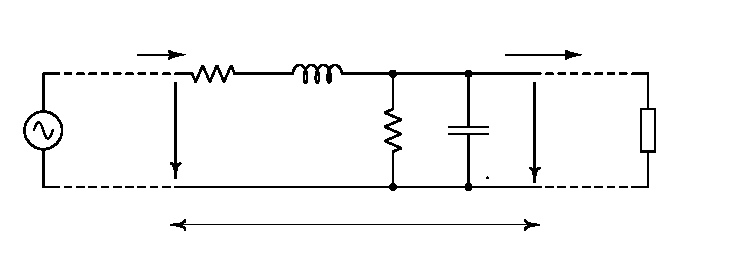
\includegraphics[scale=1.25]{vedenie}\\
   % translate x=237 y=229 scale 0.28
   \putbox{2.43in}{1.52in}{1.20}{\llaL}%
   \putbox{4.00in}{1.64in}{1.20}{\llaidi}%
   \putbox{1.52in}{1.52in}{1.20}{\llaR}%
   \putbox{3.25in}{0.97in}{1.20}{\llaG}%
   \putbox{3.88in}{0.97in}{1.20}{\llaC}%
   \putbox{0.42in}{0.81in}{1.20}{\llaGen}%
   \putbox{5.38in}{0.81in}{1.20}{\llaZat}%
   \putbox{4.36in}{0.81in}{1.20}{\llaudu}%
   \putbox{1.36in}{0.81in}{1.20}{\llau}%
   \putbox{1.09in}{1.64in}{1.20}{\llai}%
   \putbox{2.58in}{0.14in}{1.20}{\lladx}%
   } % close 'parbox'
   } % close 'scalebox'
   \vspace{-\baselineskip} % this is not necessary, but looks better

	\caption{Element dĺžky $\dif x$ vedenia s rozloženými parametrami.}
	\label{fig:vedenie}
\end{figure}
Z Kirchhoffových rovníc a následného separovania premenných (rovnica zvlášť pre $(i(x,t)$ resp. $u(x,t)$) vyplývajú známe telegrafné rovnice.
Pre výrazné matematické zjednodušenie (prechod od parciálnych k obyčajným diferenciálnym rovniciam) je možné hoci aj na úkor všeobecnosti zaviesť technicky zmysluplný predpoklad harmonických priebehov veličín a namiesto časových derivácii a integrácii využiť symbolickú metódu koplexného operátora $j \omega$. Potom:

\begin{subequations} \label{eq:vedenie_harm_kirch}
	\begin{align}
	\dxdtp{\cpx{U}}{x} \dif x = R \cdot \cpx{I} \cdot \dif x + j\omega L \cdot \cpx{I} \cdot \dif x\\
	\dxdtp{\cpx{I}}{x} \dif x = G \cdot \cpx{U} \cdot \dif x + j\omega C \cdot \cpx{U} \cdot \dif x
\end{align}
\end{subequations}

Vynásobením rovníc (\ref{eq:vedenie_harm_kirch}) faktorom $\frac{1}{\dif x}$ dostávame:

\begin{subequations} \label{eq:vedenie_harm_duidx}
	\begin{align}
		\dxdtp{\cpx{U}}{x} = (R + j\omega L) \cdot \cpx{I} = \cpx{Z} \cdot \cpx{I} \label{eq:vedenie_harm_duidx_U'=Z.I}\\
		\dxdtp{\cpx{I}}{x} = (G + j\omega C) \cdot \cpx{I} = \cpx{Y} \cdot \cpx{U} \label{eq:vedenie_harm_duidx_I'=Y.U}
\end{align}
\end{subequations}

Vyjadrením $\dxdtp{\cpx{U}}{x} = \dxdtp{^2\cpx{I}}{x^2} \cdot \frac{1}{\cpx{Y}}$ z (\ref{eq:vedenie_harm_duidx_I'=Y.U}) a dosadením do (\ref{eq:vedenie_harm_duidx_U'=Z.I}) a naopak dostávame \textbf{telegrafné rovnice pre harmonické priebehy}:

\begin{subequations} \label{eq:telegraf_harm}
	\begin{align}
		\dxdtp{^2\cpx{I}}{x^2} = \cpx{Z}\cpx{Y} \cdot \cpx{I} \label{eq:telegraf_harm_i}\\
		\dxdtp{^2\cpx{U}}{x^2} = \cpx{Z}\cpx{Y} \cdot \cpx{U} \label{eq:telegraf_harm_u}
	\end{align}
\end{subequations}
Riešením rovnice $\dxdtp{^2\cpx{U}}{x^2} - \cpx{Z}\cpx{Y} \cdot \cpx{U} = 0$, tj. (\ref{eq:telegraf_harm_u}) je:

\begin{equation}
	\cpx{U}(x) = \cpx{U}_{0+} \cdot e^{\sqrt{\cpx{Z}\cpx{Y}} \cdot x} + \cpx{U}_{0-} \cdot e^{-\sqrt{\cpx{Z}\cpx{Y}} \cdot x}
	\label{eq:telegraf_riesenie_u}
\end{equation}

Komplexné časovo natáčajúce sa fázory $\cpx{U}_{0+}$ a  $\cpx{U}_{0+}$ predstavujú harmonické vlnenie, exponenciálne členy predstavujú útlm amplitúdy pozdĺž vedenia, a to v doprednom resp. spätnom smere. Hovoríme o priamej a odrazenej vlne. Výsledná vlna je superpozíciou priamej a odrazenej vlny.

Dosadením riešenia (\ref{eq:telegraf_riesenie_u}) do (\ref{eq:vedenie_harm_duidx_U'=Z.I}) získavame výraz pre prúdovú vlnu:

\begin{equation}
	\cpx{I}(x) = \frac{1}{\cpx{Z}} \dxdtp{\cpx{U}}{x} = \frac{1}{\cpx{Z}} \sqrt{\cpx{Z}\cpx{Y}} \left( \cpx{U}_{0+} \cdot e^{\sqrt{\cpx{Z}\cpx{Y}} \cdot x} - \cpx{U}_{0-} \cdot e^{-\sqrt{\cpx{Z}\cpx{Y}} \cdot x} \right)
	\label{eq:telegraf_harm_riesenie_i}
\end{equation}

Výrazu
\begin{equation}
	\sqrt{\frac{\cpx{Z}}{\cpx{Y}}} = \cpx{Z}_0
	\label{eq:char_impedancia}
\end{equation}
sa hovorí \textbf{charakteristická (vlnová) impedancia vedenia}.

Potom výrazy pre napäťovú (\ref{eq:telegraf_riesenie_u}) a prúdovu (\ref{eq:telegraf_harm_riesenie_i}) vlnu nadobudnú tvar:

\begin{subequations} 
	\label{eq:telegraf_harm_riesenia_obe}
	\begin{align}
		\cpx{U}(x) = \cpx{U}_{0+} \cdot e^{\sqrt{\cpx{Z}\cpx{Y}} \cdot x} + \cpx{U}_{0-} \cdot e^{-\sqrt{\cpx{Z}\cpx{Y}} \cdot x}
	\label{eq:telegraf_harm_riesenia_obe_u}\\
		\cpx{I}(x) = \frac{1}{\cpx{Z}_0} \left( \cpx{U}_{0+} \cdot e^{\sqrt{\cpx{Z}\cpx{Y}} \cdot x} - \cpx{U}_{0-} \cdot e^{-\sqrt{\cpx{Z}\cpx{Y}} \cdot x} \right)
	\label{eq:telegraf_harm_riesenia_obe_i}
	\end{align}
\end{subequations}

Výrazy $\cpx{U}_{0+}$, $\cpx{U}_{0-}$ predstavujú okrajové podmienky riešenia To všeobecne neznamená že by priamo vyjadrovali konkrétnu fyzikálnu alebo merateľnú kvantitu ako napr. vstupné alebo výstupné napätie na vedení. Dosadením známeho vstupného ($x=0$) alebo výstupného ($x=l$) napätia a prúdu do (\ref{eq:telegraf_harm_riesenia_obe}) sa však dajú jednoznačne vyjadriť.

Zámerom je \uv{nastavenie} okrajových podmienok tak, aby nedochádzalo na vedení k odrazom.
Výstupné napätie považujme za dané; výstupný prúd bude potom určený výstupnou impedanciou: $i_{výst} = \frac{u_{výst}}{Z_{výst}}$, resp.:
\begin{equation}
	\cpx{I}_{výst} = \frac{\cpx{U}_{výst}}{\cpx{Z}_{výst}}
	\label{eq:Ivyst=Uvyst/Zvyst}
\end{equation}

Dosadením daného výstupného napätia $\cpx{U}(l) = \cpx{U}_{výst}$ do (\ref{eq:telegraf_harm_riesenia_obe_u}) dostávame:
\begin{equation}
	\cpx{U}_{výst} = \cpx{U}_{0+} \cdot e^{\sqrt{\cpx{Z}\cpx{Y}} \cdot l} + \cpx{U}_{0-} \cdot e^{-\sqrt{\cpx{Z}\cpx{Y}} \cdot l}
	\label{eq:telegraf_Uvyst}
\end{equation}

Ďalej dosadením (\ref{eq:telegraf_Uvyst}) do (\ref{eq:Ivyst=Uvyst/Zvyst}) vyjadríme:
\begin{equation}
	\cpx{I}_{výst} = \frac{1}{\cpx{Z}_{výst}} \left( \cpx{U}_{0+} \cdot e^{\sqrt{\cpx{Z}\cpx{Y}} \cdot l} + \cpx{U}_{0-} \cdot e^{-\sqrt{\cpx{Z}\cpx{Y}} \cdot l} \right)
	\label{eq:telegraf_Ivyst=Uvyst/Z_vyst}
\end{equation}

a zároveň platí telegrafná rovnica (\ref{eq:telegraf_harm_riesenia_obe_i}):
\begin{equation}
	\cpx{I}_{výst} = \frac{1}{\cpx{Z}_0} \left( \cpx{U}_{0+} \cdot e^{\sqrt{\cpx{Z}\cpx{Y}} \cdot l} - \cpx{U}_{0-} \cdot e^{-\sqrt{\cpx{Z}\cpx{Y}} \cdot l} \right)
	\label{eq:telegraf_Ivyst}
\end{equation}

Porovnaním pravých strán (\ref{eq:telegraf_Ivyst=Uvyst/Z_vyst}) a (\ref{eq:telegraf_Ivyst}) dostávame vzťah:

\begin{equation}
	\frac{1}{\cpx{Z}_{výst}} \left( \cpx{U}_{0+} \cdot e^{\sqrt{\cpx{Z}\cpx{Y}} \cdot l} + \cpx{U}_{0-} \cdot e^{-\sqrt{\cpx{Z}\cpx{Y}} \cdot l} \right)
	=
	\frac{1}{\cpx{Z}_0} \left( \cpx{U}_{0+} \cdot e^{\sqrt{\cpx{Z}\cpx{Y}} \cdot l} - \cpx{U}_{0-} \cdot e^{-\sqrt{\cpx{Z}\cpx{Y}} \cdot l} \right)
	\label{eq:Ivyst_prave_strany}
\end{equation}

I bez toho, aby sme vyjadrovali výrazy $\cpx{U}_{0+}$, $\cpx{U}_{0-}$ sa dá z rovnice (\ref{eq:Ivyst_prave_strany}) usúdiť chovanie na vedení za určitých hraničných podmienok.

Pri výstupe vedenia naprázdno bude $Z_{výst} \to \infty$, čiže výraz na pravej strane  (\ref{eq:Ivyst_prave_strany}) bude nulový. Potom aj ľavá strana bude rovná nule a na vedení vzniká stojaté vlnenie \footnote{koeficient odrazu definovaný ako pomer odrazenej a priamej vlny (v každom bode pozdĺž osi x) je na konci vedenia naprázdno rovný jednotke.}. Tejto situácii približne zodpovedá pripojenie vedenia na $1\un{M\Ohm}$ vstupný odpor osciloskopu.

Pokiaľ požadujeme na konci vedenia neprítomnosť odrazov, pričom primárne parametre vedenia sú dané jeho konštrukciou (u koaxiálneho kábla $Z_0 = 50\Ohm$) a dĺžka $l$ je pevná, potom je nutné upraviť vstupnú impedanciu osciloskopu, a to takým spôsobom, aby mala rovnica sústavy riešenie práve vtedy, keď $\cpx{U}_{0-} = 0$.
 $\cpx{U}_{0-} = 0$ preto dosadíme do (\ref{eq:Ivyst_prave_strany}) a získavame známy vzťah pre prispôsobenie na výstupe vedenia:
\begin{equation}
	\cpx{Z}_{výst} = 
	\cpx{Z}_0 \frac{\cpx{U}_{0+}\cdot e^{\sqrt{\cpx{Z}\cpx{Y}}\cdot l}}{\cpx{U}_{0+}\cdot e^{\sqrt{\cpx{Z}\cpx{Y}}\cdot l}} =
	\cpx{Z}_0 = 50\un{\Ohm}
	\label{eq:Zvyst=Z0}
\end{equation}

Obdobným spôsobom je možné odvodiť ekvivalentný vzťah pre prispôsobenie na vstupe vedenia.
